   
\documentclass[12pt, oneside]{report}
\usepackage{amsfonts, epsfig, setspace,amssymb,amsmath, textcomp} %natbib,}
\usepackage{graphics}
\usepackage{multicol}
\usepackage[document]{ragged2e}
\usepackage{wrapfig, blindtext}
\usepackage{subcaption}
\usepackage{tabu}

\oddsidemargin 10pt \evensidemargin 1ex \textwidth 6.6in \textheight
9.2in \topmargin -0.5in \baselineskip 15pt

\newsavebox{\savepar}
\newenvironment{boxit}{\begin{center}\begin{lrbox}{\savepar}
\begin{minipage}[t]{13cm} }
{\end{minipage}\end{lrbox}\fbox{\usebox{\savepar}}\end{center}}


\newtheorem{example}{\bf Example}[section]
\newtheorem{examples}{\bf Examples}[section]
\newtheorem{corollary}{\bf Corollary}[section]
\newtheorem{remark}{\bf Remark}[section]
\newtheorem{remarks}{\bf Remarks}[section]
\newtheorem{lemma}{\bf Lemma}[section]
\newtheorem{theorem}{\bf Theorem}[section]
\newtheorem{proposition}{\bf Proposition}[section]
\newtheorem{definition}{\bf Definition}[section]
\newtheorem{notation}{\bf Notation}[section]
\newtheorem{question}{\bf Question}
\newtheorem{property}{\bf Property}
\numberwithin{equation}{section}


% \newenvironment{proof}[1][Proof]{\begin{trivlist}
% \item[\hskip \labelsep {\bfseries #1}]}{\end{trivlist}}
% 
% \newcommand{\qed}{\nobreak \ifvmode \relax \else
%       \ifdim\lastskip<1.5em \hskip-\lastskip
%       \hskip1.5em plus0em minus0.5em \fi \nobreak
%       \vrule height0.75em width0.5em depth0.25em\fi}

\linespread{1.5}




\begin{document}


\thispagestyle{empty}
\begin{center}
{\large \bf B.Tech. Project Report\\ }
\vspace{0.5cm} {\large  on\\ }
\vspace*{0.06in} {\LARGE \bf Unmanned Arial Vehicle \\}
\vspace*{0.1in} {\LARGE \bf \textit{\underline{Project Sudarshana}} \\} \vspace*{0.1in}
\vspace{0.1cm} {\large  and\\ }
\vspace*{0.01in} {\LARGE \bf Home Automation \\}
% { Thesis}\\
% {\large Submitted in Partial Fulfillment of the Requirements}\\
% {\large for the Degree of}\\
% \vspace{0.1in}
% {\Large \bf Doctor of Philosophy}\\
\vspace{0.2in}
{ Submitted by} \\
\vspace{0.1in}
{\Large \bf Hari Pad Rajak } \\
{\large  201451001}\\
\vspace{0.1in}
{\Large \bf Vishal Nagarale } \\
{\large  201451004}\\
\vspace{0.2in}
{\large  under the supervision of\\ }
%{\bf Supervisor: } \\
\vspace{.1in}
{\Large \bf Prof. K. K. Jha } \\
\vspace{.1in}
%\vspace{.1in}
%{\bf \large Mentor: } \\
%\vspace{.1in}
%{\Large \bf Name (for off-campus BTP) } \\
\vspace{0.1in}
% \begin{figure}[h]
% {\centering 
% \resizebox*{1.5in}{1.2in}{\includegraphics{iitblogoFundoo.ps}}
% \par}
% \end{figure}
% \begin{figure}[ph]
% \centering \epsfysize = 1.7in
% \mbox{ \epsfbox{logo.png} }
% \epsfbox{IITB.pdf}
% \end{figure}
%\begin{center}
\vspace*{2cm}

\includegraphics[width=3cm]{logo}\\
%\end{center}
\vspace{0.1in}
%{\large \bf DEPARTMENT OF MATHEMATICS \\
{\large INDIAN INSTITUTE OF INFORMATION TECHNOLOGY, VADODARA \\
 April 2018}
\end{center}
\newpage



\thispagestyle{empty}

%\end{center}
\newpage
%\include{declaration}
\centering{\bf\Large Declaration\\ }
\justify
We, Hari Pad Rajak and Vishal Nagarale, declare that this written submission represents our ideas in our own words and where
other$'$s ideas or words have been included, We have adequately cited and referred the
original sources. We also declare that We have adhered to all principles of academic honesty
and integrity and have not mispresented or fabricated any idea/data/fact/source
in our submission. We fully understand that any violation of the above will cause for disciplinary
action by the institute and can also evoke penal action from the sources which have thus
not been properly cited or from whom proper permission has not been obtained.\\
\vspace{1cm}
%\hspace*{\fill}
%\hfill {(Signature)}\\
%\hfill{Hari Pad Rajak}\\
%\hfill{201451001}
%\hfill
%\hfill {(Signature)}\\
%\hfill{Vishal Nagarale}\\
%\hfill{201451004}
%\hspace*{\fill}

\begin{multicols}{2}
\begin{minipage}{\textwidth}

Hari Pad Rajak \\
201451001\\

\vspace*{\fill}
\vspace{1cm}
Date: 27/04/2018

\end{minipage}
Vishal Nagarale \\
201451004

\end{multicols}



\newpage
\pagenumbering{roman}

\centerline{{\bf {\large Abstract}}}
\justify
Artificial Intelligence is the future of today’s world. Drones, technically known as unmanned
aerial vehicles (UAVs), are one such form of artificial intelligence which shall change the
course of technology and the world soon. Drone technology has immense potential, not only
for technological and economic growth globally but also for security reasons of the nation.
Currently, in India, on a major scale, we don't have any technology used for security which
is based on drones. So we come up with the idea of using drones for our day-to-day life
surveillance and security. The drone will be one of the cheapest drones used for security and
has a special feature of an electric gun which can be used in case of emergency. The main
problem of our society is the acknowledgment of crime happened much later than the crime,
that’s why many of proofs got destroyed due to any reason. The drone surveillance gives a
better eye on each and every part of the society and helps to reduce the crime rate. We try to
build a drone with face recognition technology embedded in it also with the electric gun so that
if any suspect found by drone it will immediately take appropriate action about it. The result
of it will be the city will be under surveillance for 24x7 without using a lot of manpower and
resources, the drones are itself self- sufficient to have an eye on the society and immediately
inform the police if anything went wrong in the city. We are living in the 21st Century where
automation (industrial or home) plays an important role in human life. So home automation
is the great move towards the future where all the things now become automated. It would make the huge impact in people’s lives and make them easier for the human being.


\vspace{1cm}



\noindent 
\tableofcontents

\newpage
\pagenumbering{arabic}

\begin{chapter}{Introduction}
Our objective for the project is to build a quadcopter that is capable of stable flight with security surveillance with the help of camera embedded on to it. More specifically our goal is to develop a surveillance system which can monitor the city 24x7 with the help of self-sufficient drone having the camera mounted on to it. We also developed our remote control which is much cheaper than market value and mostly does the same work as other remote controllers do. While there are many open source programs which give transmitter and receiver Arduino code but we wanted to develop the code ourselves in order to learn more about what are the actual values which are responsible for the drone to take off. The purpose of the report is to describe results of the project and the steps those were necessary to reach the result.\\
The next objective is to automate Prof. Kamal sir's lab with the help of minimal electronic components without complex soldering and simple and flexible design.

\end{chapter}


\begin{chapter}{Essentials for Project}
 
%\begin{enumerate}
%\end{enumerate}
\section{Quadcopter}
Every radio-controlled (RC) requires, following components: a frame, motors with propellers, Electronic speed controller (ESC), a battery, a radio receiver, a flight controller. This section will discuss the function of each component.

\subsection{Quadcopter Frame}

It provides the physical structure for the entire aircraft. It joins the motors to the rest of components and houses all the other components. The frame must be large enough to avoid the collisions between propellers and not too large and therefore too heavy for the motors.
%\begin{wrapfigure}{r}{0.25\textwidth} %this figure will be at the right
\begin{figure}
	\center
    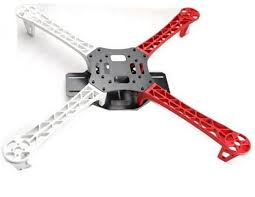
\includegraphics[width=0.35\textwidth]{frame}
    \caption{Quadcopter Frame}
\end{figure}    
    
%\end{wrapfigure}
%\justify

\subsection{Motors and Propellers}

The propellers spin with the help of motors to provide the quadcopters with lifting thrust. We use brush-less DC motors as they provide thrust-to-weight ratios superior to brushed DC motors. However, they required more complex ESCs.\\
There are two ratings for motors: Kv ratings and current ratings. Kv indicates that how fast the motor will spin (RPM) for 1V of the applied voltage. While the current ratings indicate max current the motors may safely draw. For this project, we select 1000Kv, 10A from REES52. \\
Propellers come in many sizes and different materials. They are measured by their pitch and diameter, in the format (diameter)x(pitch). Pitch is the measurement of how far a propeller will "travel" in one revolution. Prop selection is important to yield appropriate thrust while not overheating the motors.

%\begin{wrapfigure}{r}{0.25\textwidth} %this figure will be at the right
 %   \centering
  %  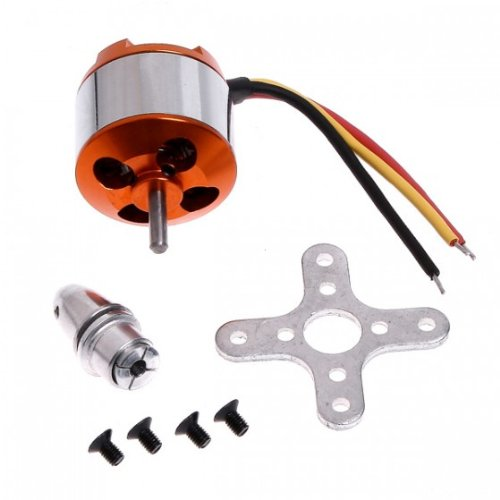
\includegraphics[width=0.25\textwidth]{motor}
%\end{wrapfigure}

\begin{figure}[h]
\center
\begin{subfigure}[hb]{0.3\textwidth}
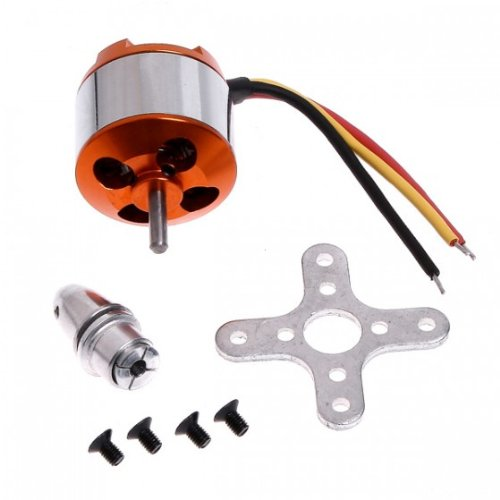
\includegraphics[width=0.8\textwidth]{motor}
\caption{Brushless motor}
\end{subfigure}
\begin{subfigure}[hb]{0.3\textwidth}
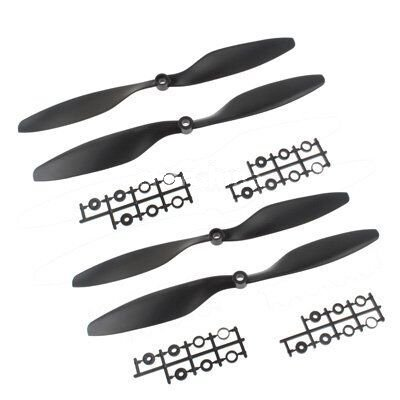
\includegraphics[width=0.8\textwidth]{prop}
\caption{Propellers}
\end{subfigure}
\end{figure}

\subsection{Electronic Speed Controllers}
Every motor needs its own electronic speed controller. They accept commands in the form of PWM signal and outputs the appropriate motor speed accordingly. Every ESC has current ratings which indicate the max current it passes to the motor without overheating. Appropriate ESCs must be chosen to ensure that they can provide enough current to the motors.
\begin{figure}[h]
\center
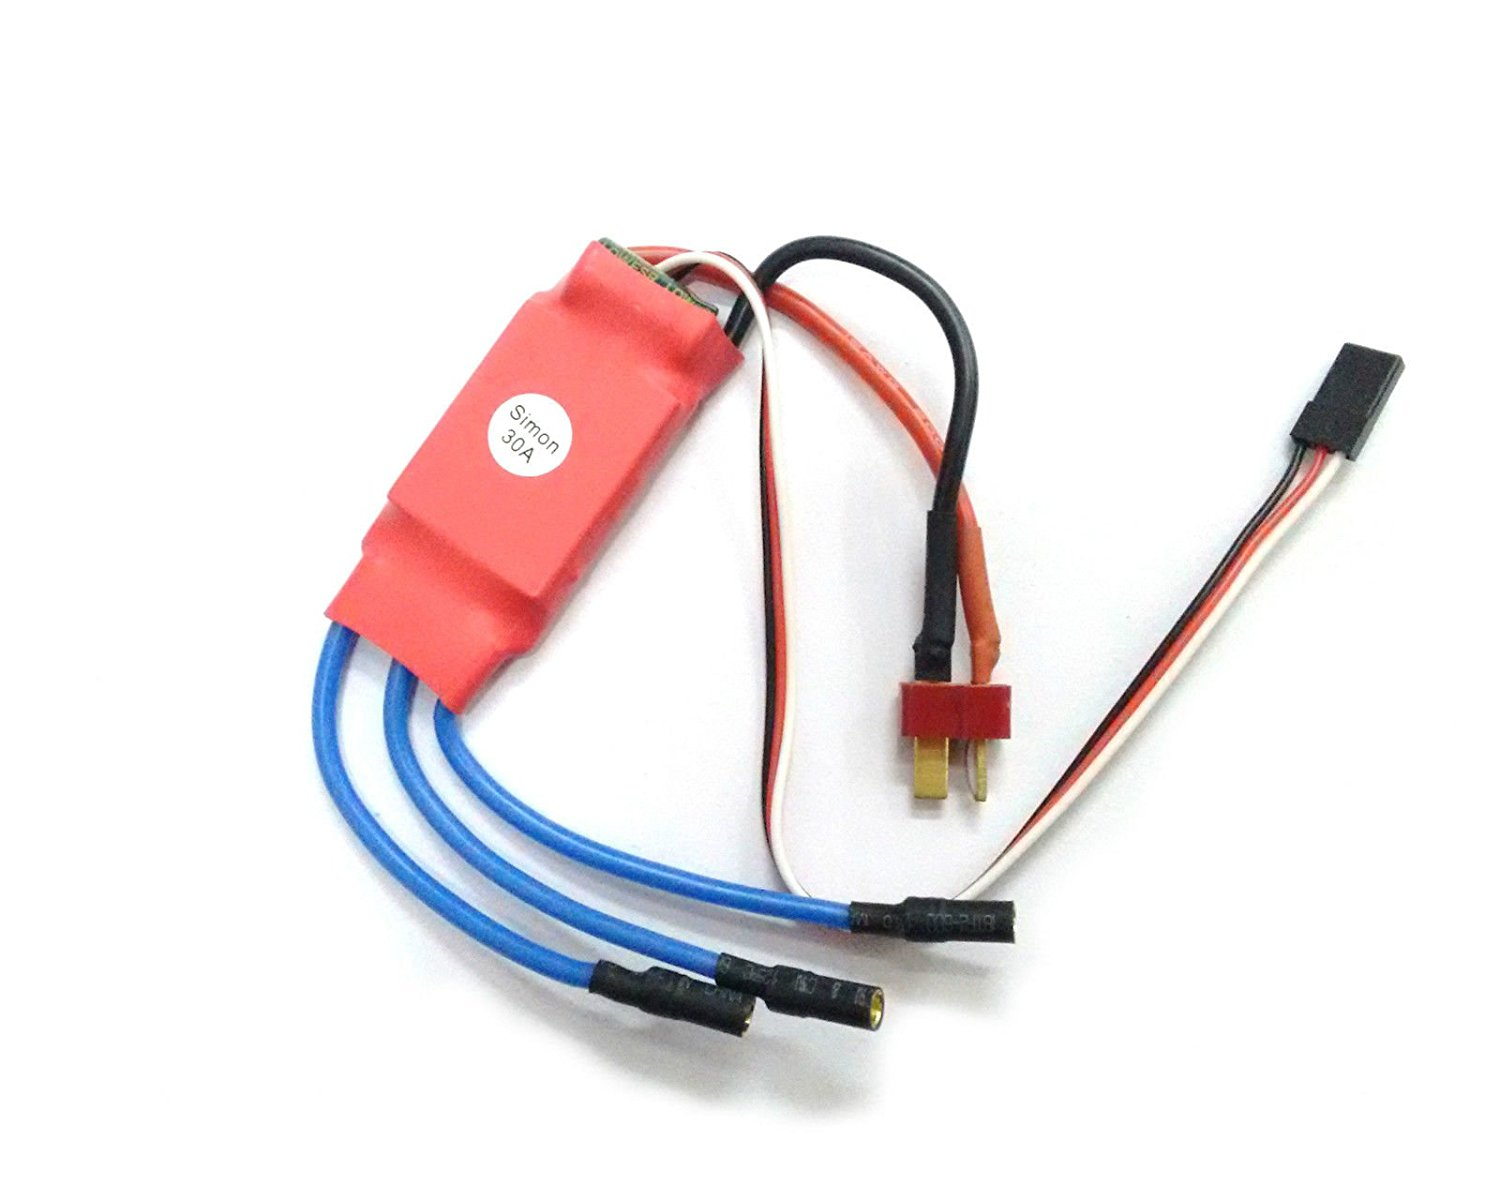
\includegraphics[width=0.35\textwidth]{esc}
\caption{Electronic Speed Controllers}
\end{figure}

\subsection{Battery and Charger}
The battery is the main and only resource of energy and provides electric power to the motors and all electronic components of the aircraft. Lithium Polymer also knew as LiPo batteries are used almost exclusively because they have high specific energy. These batteries have a capacity rating and discharge ratings. The capacity ratings which is in milliamp-hours (mAh) indicates how much current the battery may output for 1 hour. Discharge ratings indicate by the letter 'C', shows how fast the battery may be safely discharged. To get the maximum output current, multiply the C value with the capacity. We select SunRobotics LiPo rechargeable battery 11.1V | 2200mAh | 25/35C power supply. 

\begin{figure}[h]
\center
\begin{subfigure}[hb]{0.3\textwidth}
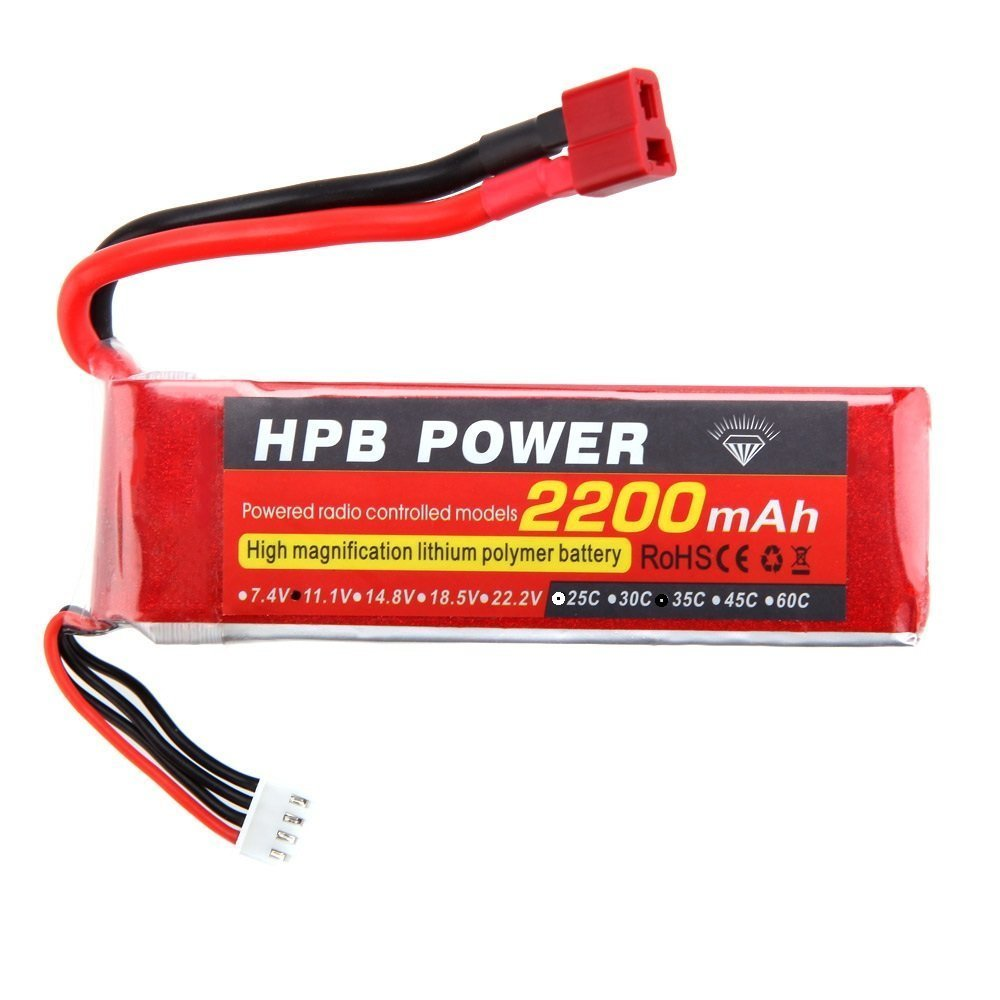
\includegraphics[width=0.8\textwidth]{battery}
\caption{LiPo Battery}
\end{subfigure}
\begin{subfigure}[hb]{0.3\textwidth}
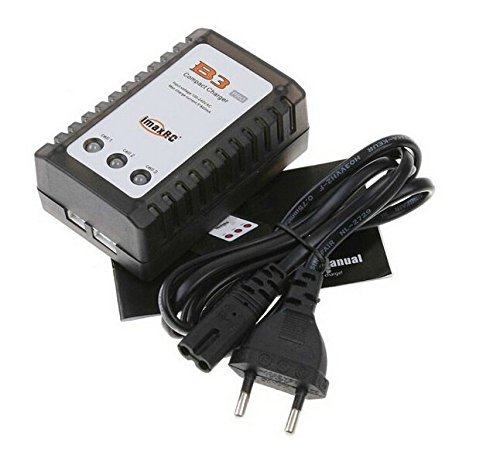
\includegraphics[width=0.8\textwidth]{charger}
\caption{LiPo Charger}
\end{subfigure}
\end{figure}

%\begin{figure}
%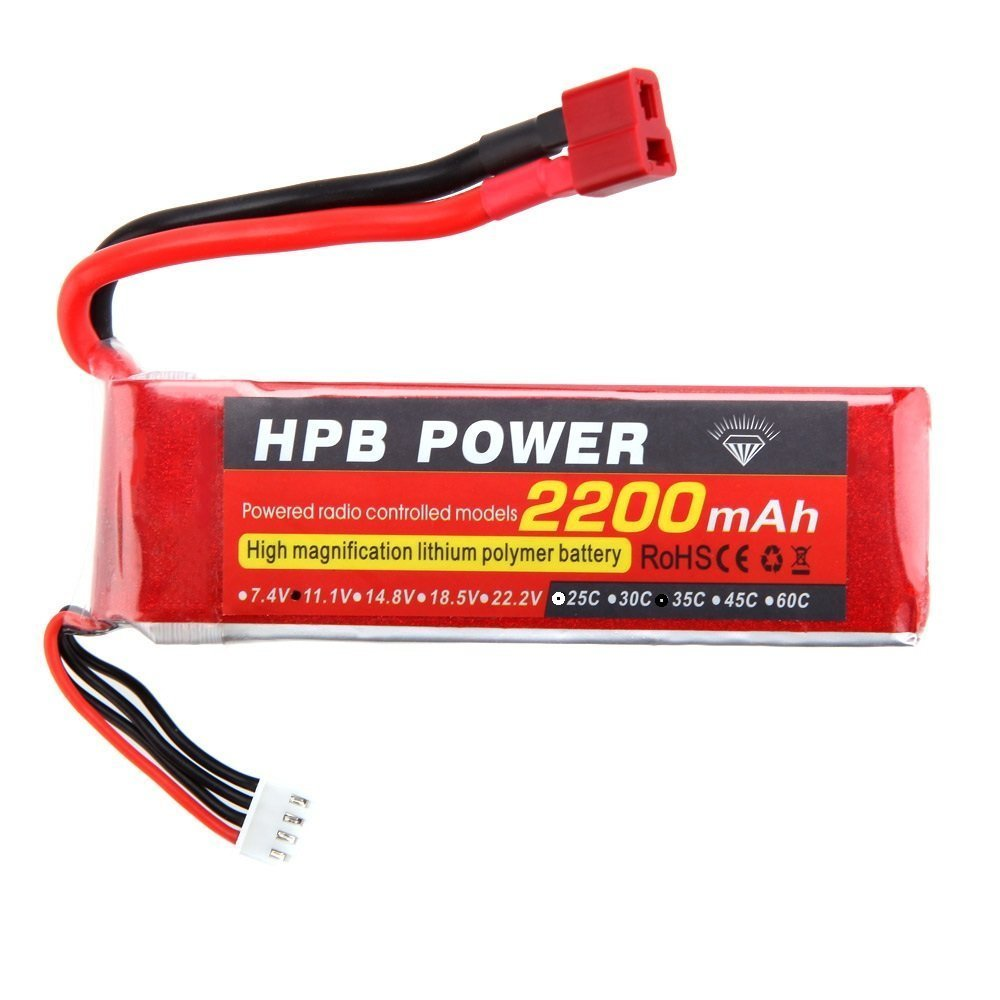
\includegraphics[width=0.35\textwidth]{battery}
%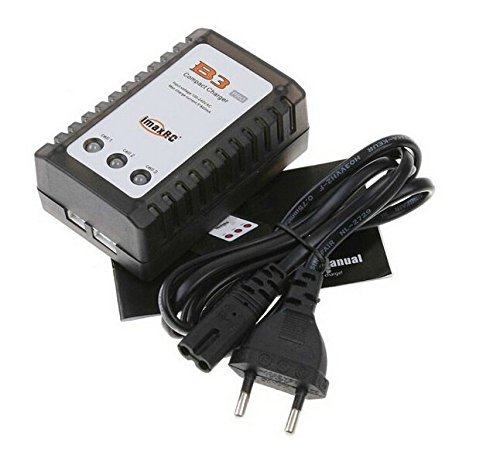
\includegraphics[width=0.35\textwidth]{charger}
%\end{figure}

The charger to charge the LiPo battery is from Robokarts balance charger for 7.4V-11.1V LiPo battery.

\subsection{Radio Transceiver \& Joysticks}
The radio receiver receives radio signals from another transceiver and converts them into control signals for each control channel i.e. for throttle, yaw, raw and pitch. Modern RC receiver works on 2.4GHz radio frequency. For this project, we choose NRF24L01 wireless transceiver RF transceiver module 2.4GHz with antenna, compatible with Arduino and Rasberry Pi.\\
Joysticks are required to make a remote control which controls the quadcopter. As we are working on Arduino we select joystick module PS2 breakout Sensor which has 2 potentiometers and 1 switch from REES52.

\begin{figure}[h]
\center
\begin{subfigure}[hb]{0.3\textwidth}
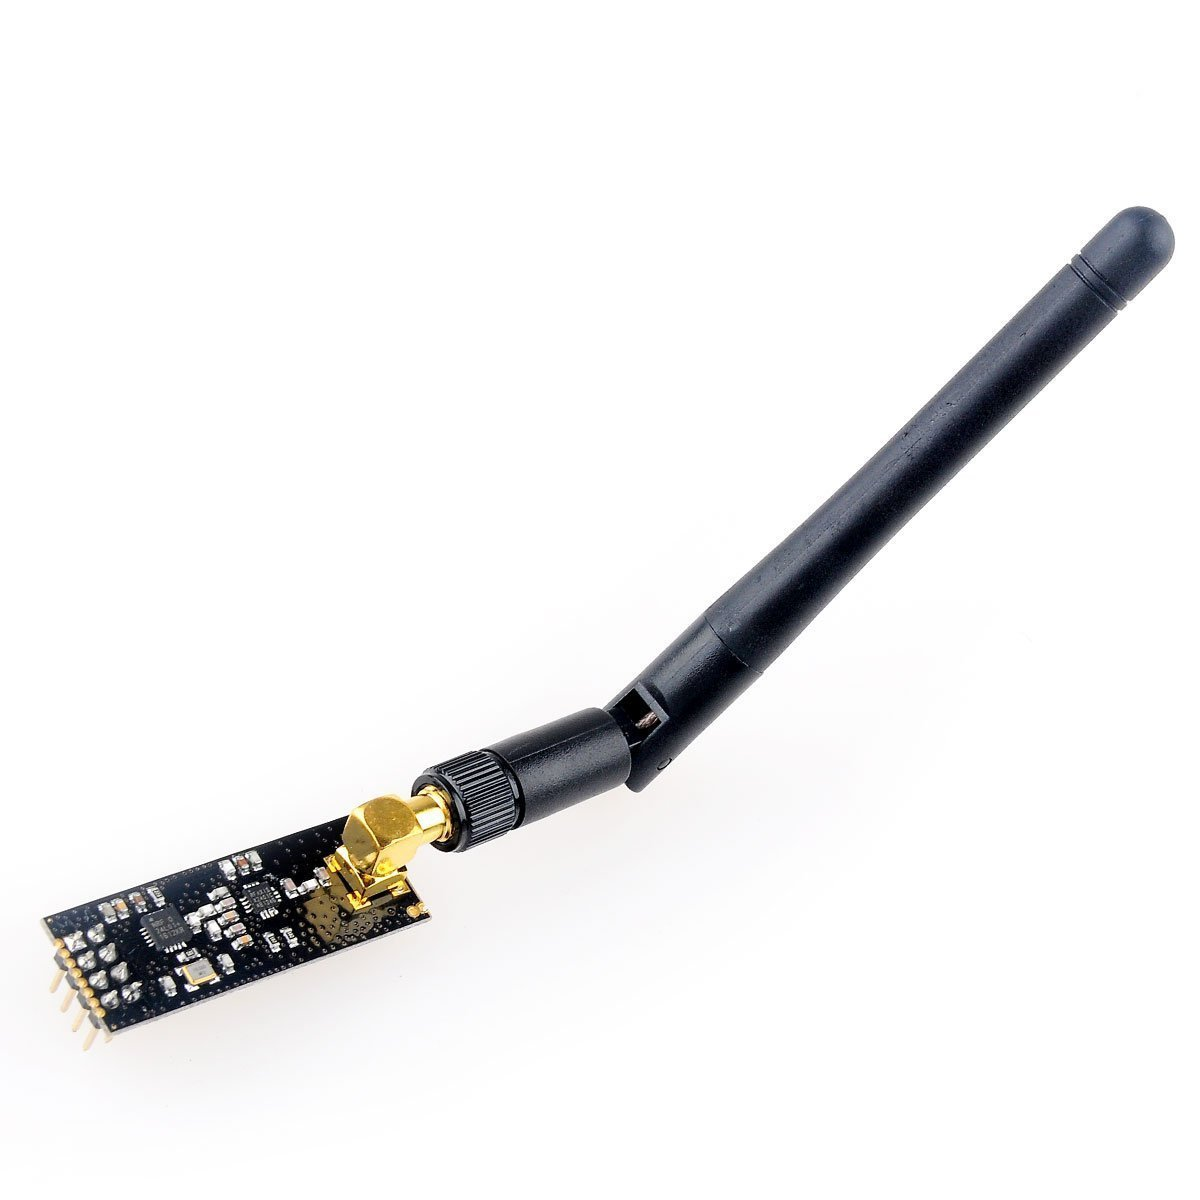
\includegraphics[width=0.8\textwidth]{transreceiver}
\caption{NRF Transceiver module}
\end{subfigure}
\begin{subfigure}[hb]{0.3\textwidth}
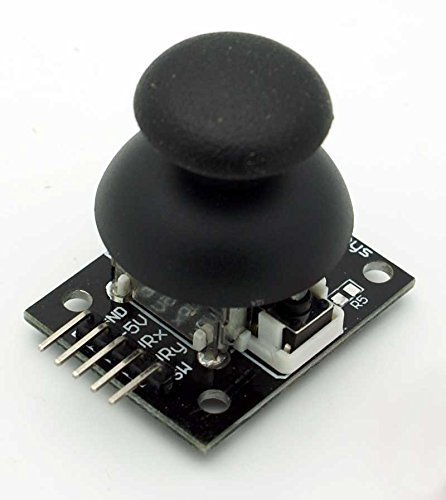
\includegraphics[width=0.7\textwidth]{joystick}
\caption{Joustick module}
\end{subfigure}
\end{figure}

%\begin{figure}
%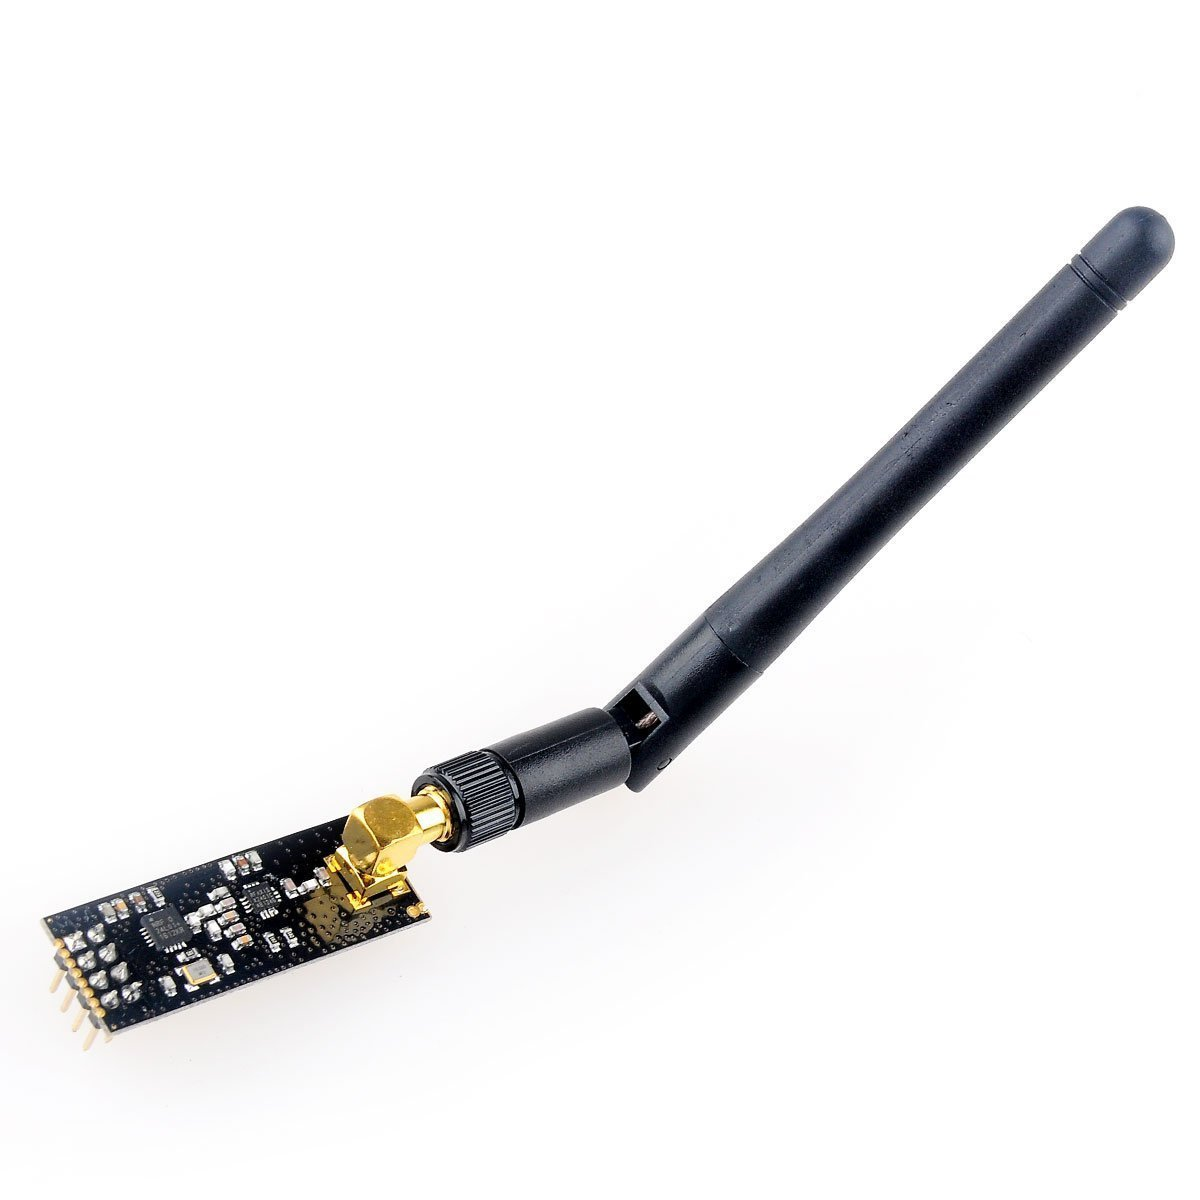
\includegraphics[width=0.35\textwidth]{transreceiver}
%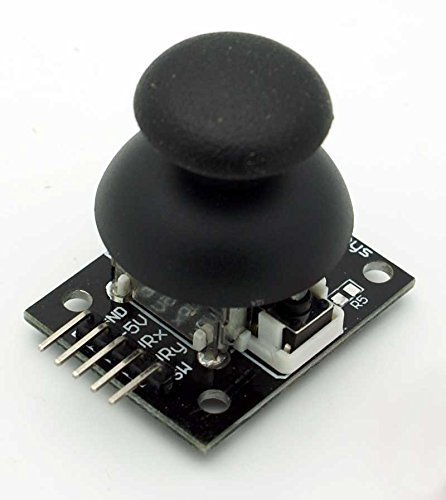
\includegraphics[width=0.35\textwidth]{joystick}
%\end{figure}

\subsection{Flight Controller}
It is known as "brain" of the quadcopter and performs the necessary operations to keep the quadcopter stable and controllable. It uses the user control commands from the receiver, combines them with readings from the altitude sensor and calculates the necessary motor output. For our project, we select KK 2.1.5 Multi-rotor LCD flight control board from Robocraze. It is purpose-made flight controller already integrated with altitude sensor and provides well-tested flight control software.\\
\begin{figure}[h]
\center
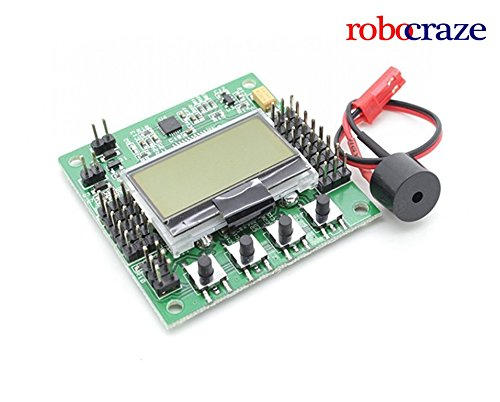
\includegraphics[width=0.35\textwidth]{flight}
\caption{KK flight controller}
\end{figure}


\subsection{Arduino Uno Board}
Actually, we need 2 Arduino boards one for the transmitter and one for the receiver. It is basically a microcontroller   (ATmega328) which operates on 5V. Input voltage recommended is 7V-12V.There are 14 digital I/O pins having the flash memory of 32 KB(ATmega328) of which 0.5 KB used by bootloader SRAM 2 KB (ATmega328)\\
\begin{figure}[h]
\center
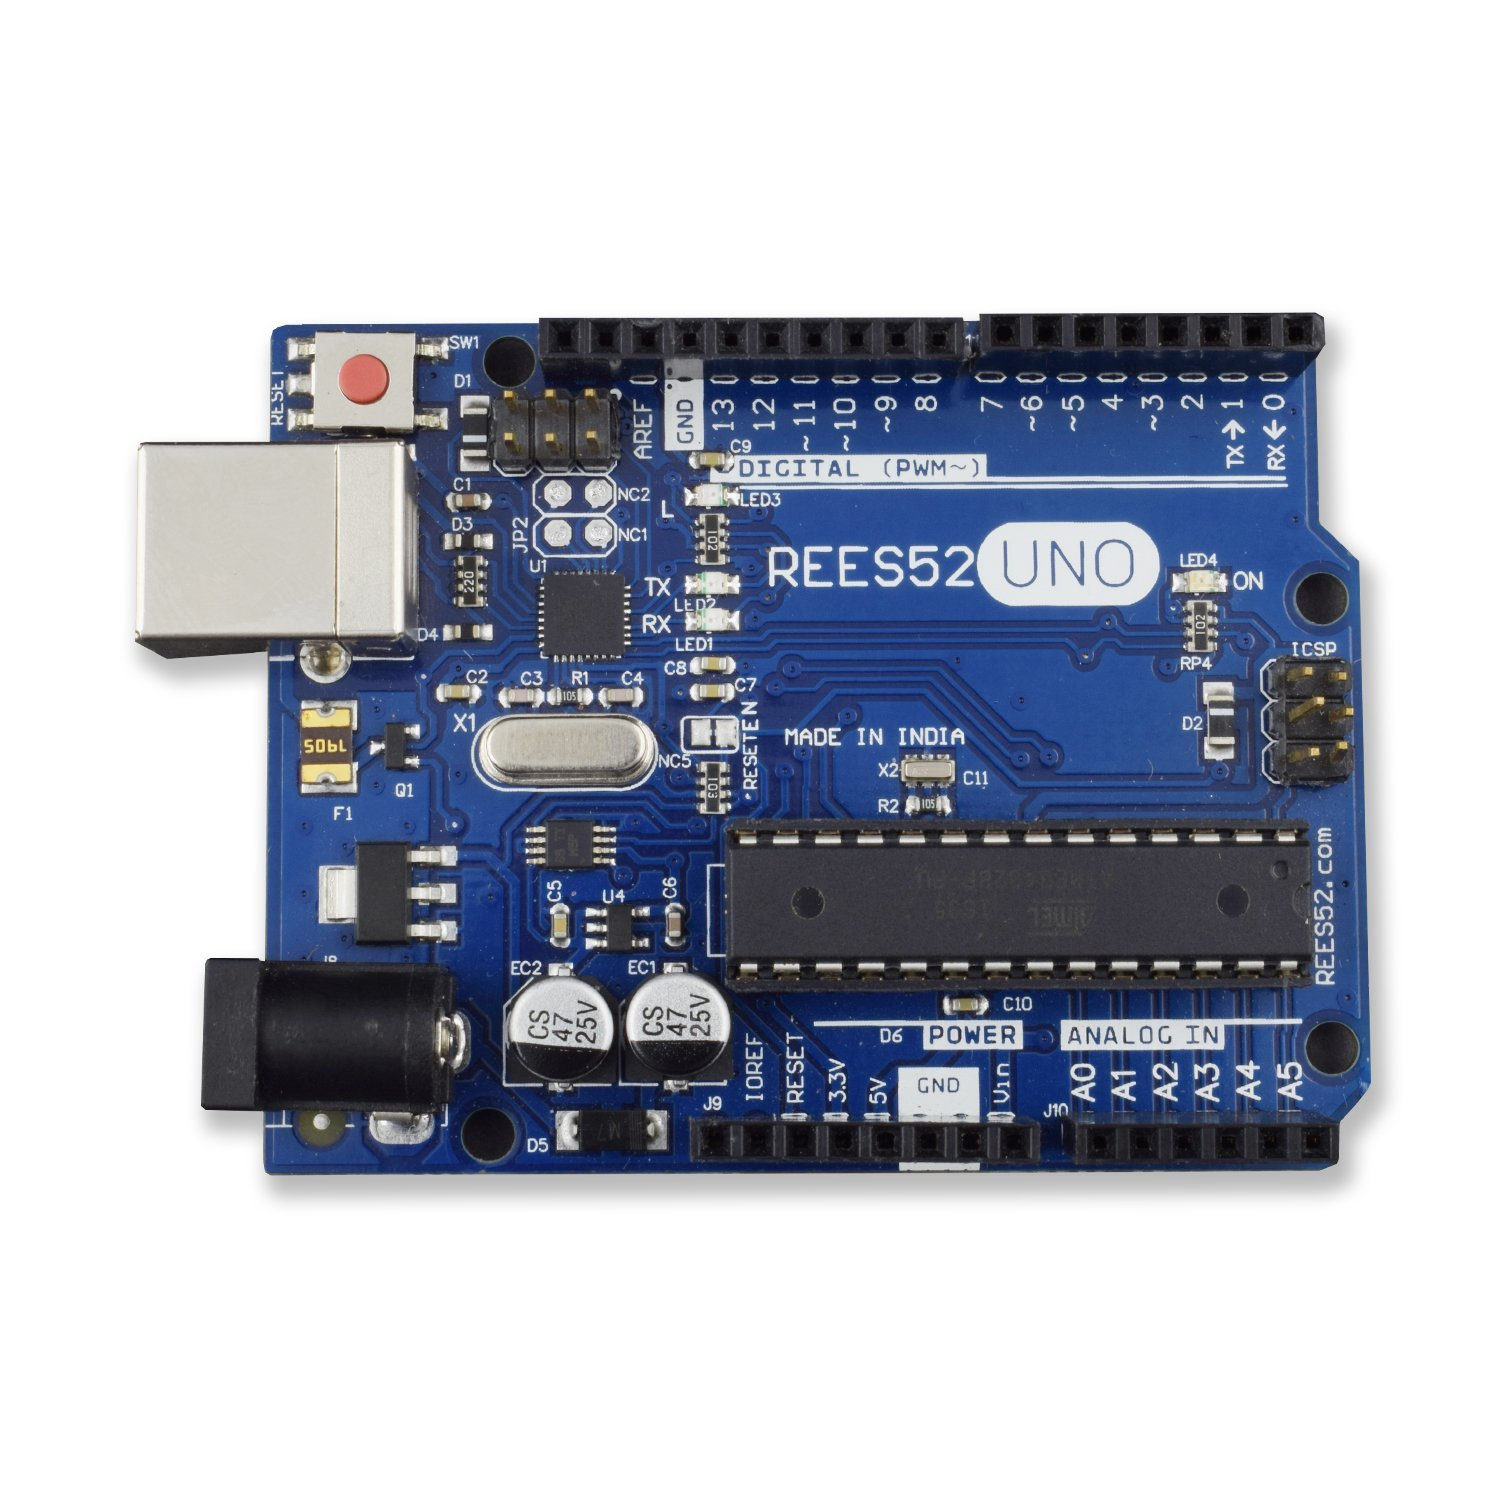
\includegraphics[width=0.25\textwidth]{arduino}
\caption{Arduino Board}
\end{figure}

\section{Home Automation}
Home automation components depend on the place where you want to automate. So for our purpose we need following things:

\subsection{Arduino Board}
The details are already mentioned in above section 2.1.7

\subsection{Bluetooth module}
The module used in this project is HC-05. As shown in the figure below it has 4-pins for VCC(5V), ground, Tx (Transmitter) and Rx (Receiver). It can enable phone and has the range of approx. 10m. \\
\begin{figure}[h]
\center
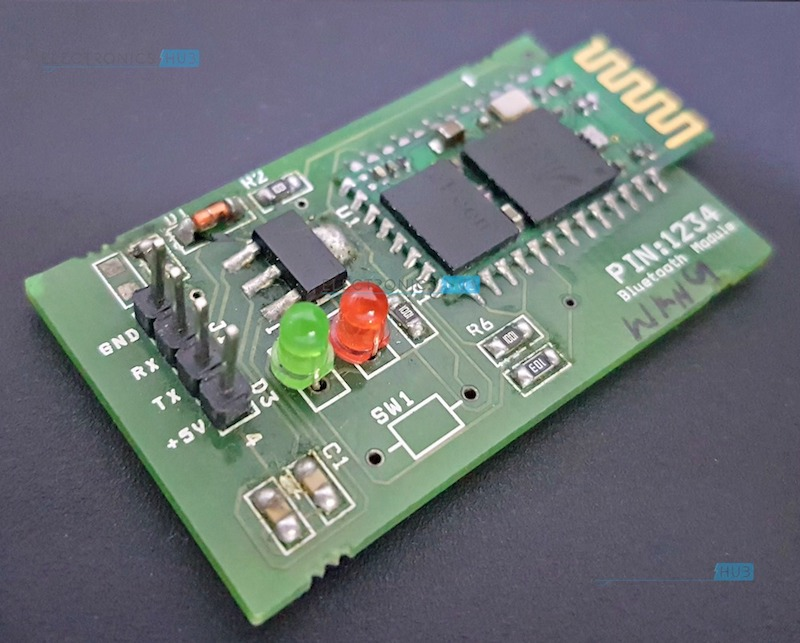
\includegraphics[width=0.35\textwidth]{Bluetooth}
\caption{HC-05 Bluetooth module}
\end{figure}

\subsection{4-Channel Relay Board}
The 4-channel relay board is used to control four different loads. It has the base current limiting resistor, flyback diode, headers etc. which are necessary components for connecting it to other devices.\\
\begin{figure}[h]
\center
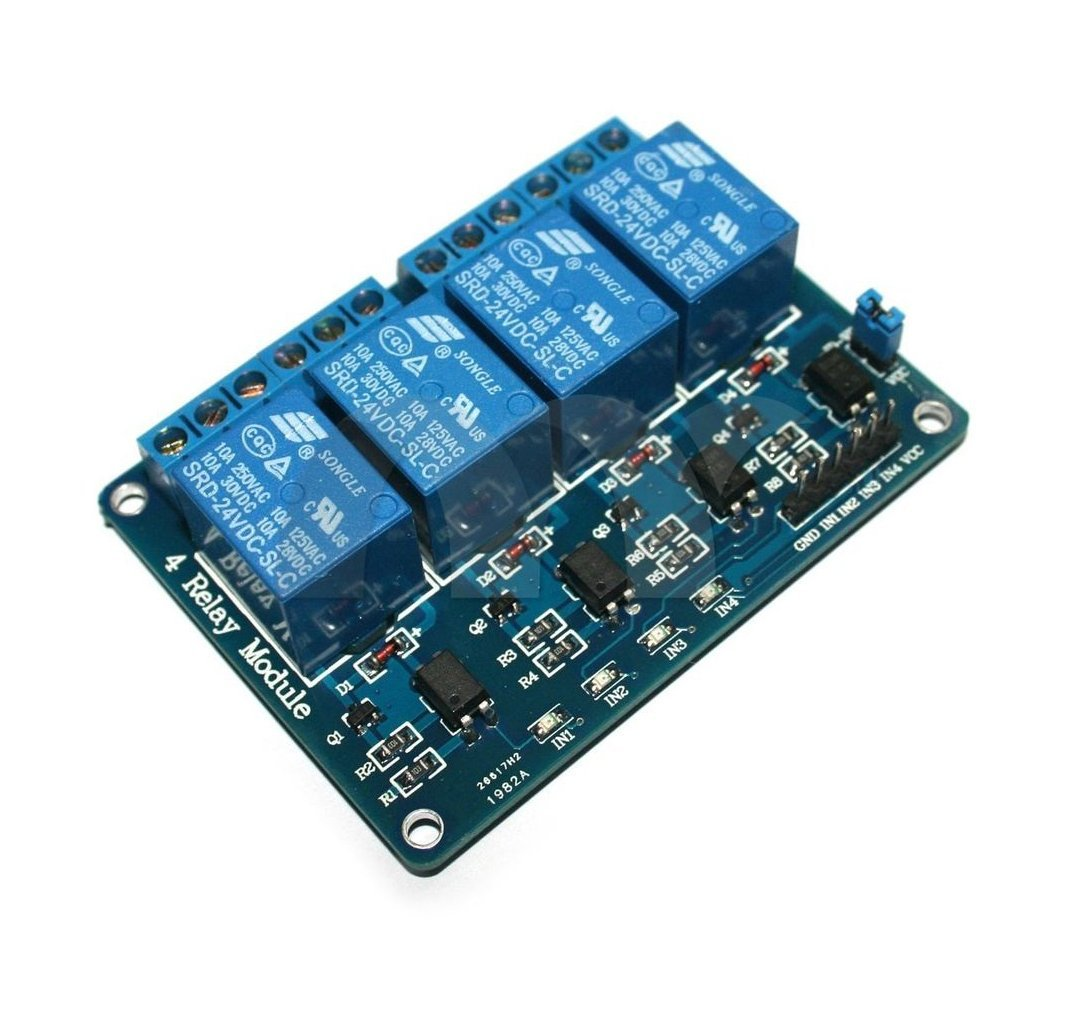
\includegraphics[width=0.45\textwidth]{relay}
\caption{4-channel relay board}
\end{figure}

\subsection{Motion Sensor}
It has wide operating voltage range: Default voltage DC 3.6V ~ 18V. In summer when the ambient temperature rises, detection distance is slightly shorter it is called temperature compensation and it is used for performance compensation.
\begin{figure}[h]
\center
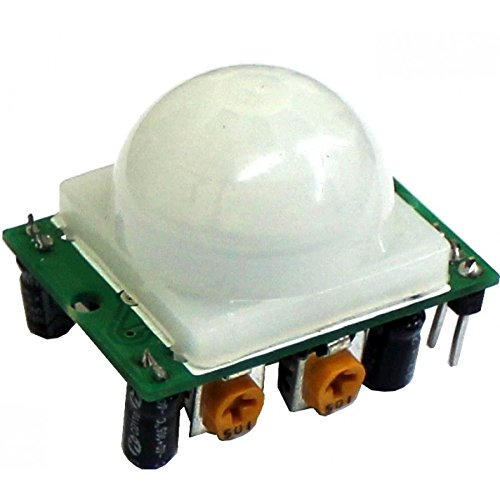
\includegraphics[width=0.35\textwidth]{motion_sensor}
\caption{Motion sensor detector module}
\end{figure}

\subsection{Connectors}
Here we need copper wires for connecting the relay board to the appliances. Copper is a good conductor of electricity and widely used in homes and industries. 

\end{chapter}


\begin{chapter}{Implementation}
\section{Procedure for Quadcopter}
\subsection{Soldering the ESCs to the Frame}
First of all, we tested the LiPo battery with the help of voltage tester and found
out that the battery is in good condition. The condition of a battery is defined
as voltage tester gives some output for the battery. (At the time of connecting the battery to tester it makes a quick buzzer noise so don’t afraid of it.)The next
thing is the charger, with LiPo battery charger firstly we have to check it without
connecting to the battery. To do so just plug-in the charger into socket board and
check if all LEDs of the charger turns into green or not, If they are green then
the charger is in good condition.If not you need to replace the charger. Now
connect the battery to the charger and on the switch all LEDs or few of them
depending on how the battery is charged turns into red. DO NOT OVERCHARGE the
battery it means as all LEDs turn into green switch off the button immediately.
\\
soldering of ESC is simple. You just need to cut the connectors (not the bullet
connectors which fits into motor but the other one) and solder them to the
board. We got the board which already has ‘positive’ \& ‘negative’ signs mark on
it but if it is not present in your frame you need to buy a Power Distribution
Board to connect all the ESCs.
\begin{figure}
\center
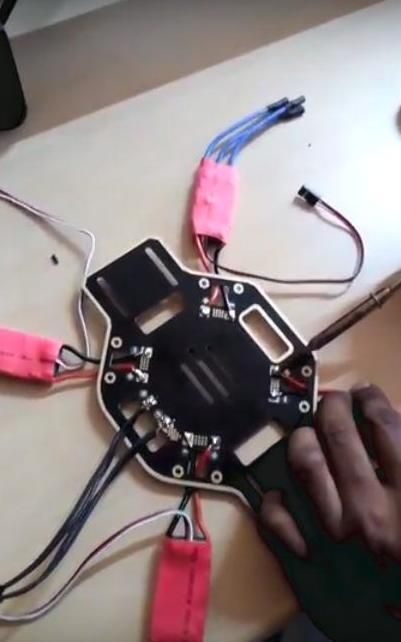
\includegraphics[width=0.35\textwidth]{base}
\caption{Drone's base}
\end{figure}

\subsection{Motor Installation with ESC}
The motors we got has something tricky in it. The cap of motor unexpectedly does not fit into the motor also the screws are short so we can’t place any vibration absorbing object between motor and drone, We need to place motor without it to get a perfect fitting. The first thing with motor is to check if they are working properly or not. To check that we took a multimeter, set it on sound mode and if it sounds BEEP as touch the wires of Multimeter to motors then it is considered to be fine. Once we are done with the motor we installed them on to the drone we move towards to the connector. We did not order the Battery connector which connects the battery to the drone and it nearly cost to Rs. 250 but we thought we can create the connector so we have cut pieces of ESC which we had removed in order to solder the ESC to the base, we solder one of them with normal wire and solder the other end of the wire with drone’s base and it works fine.\\
    The most important thing while installing the motors we need to look for the direction of the motor rotation. To do so, first of all, fix the arms of drone i.e. which part of the drone is front and which one is rare, We fixed white arms to be front and red to be rare. After that, we named it white-1, white-2, red-3, and red-4. Then according to the configuration in flight controller which will be explained later set the direction of the motor. For clockwise direction connect the ESC with Motor with same color configuration. That is the first connector of ESC goes to the first connector of the motor and likewise. But for the anti-clockwise rotation swap any two connectors and get the required result.\\
\begin{figure}
\center
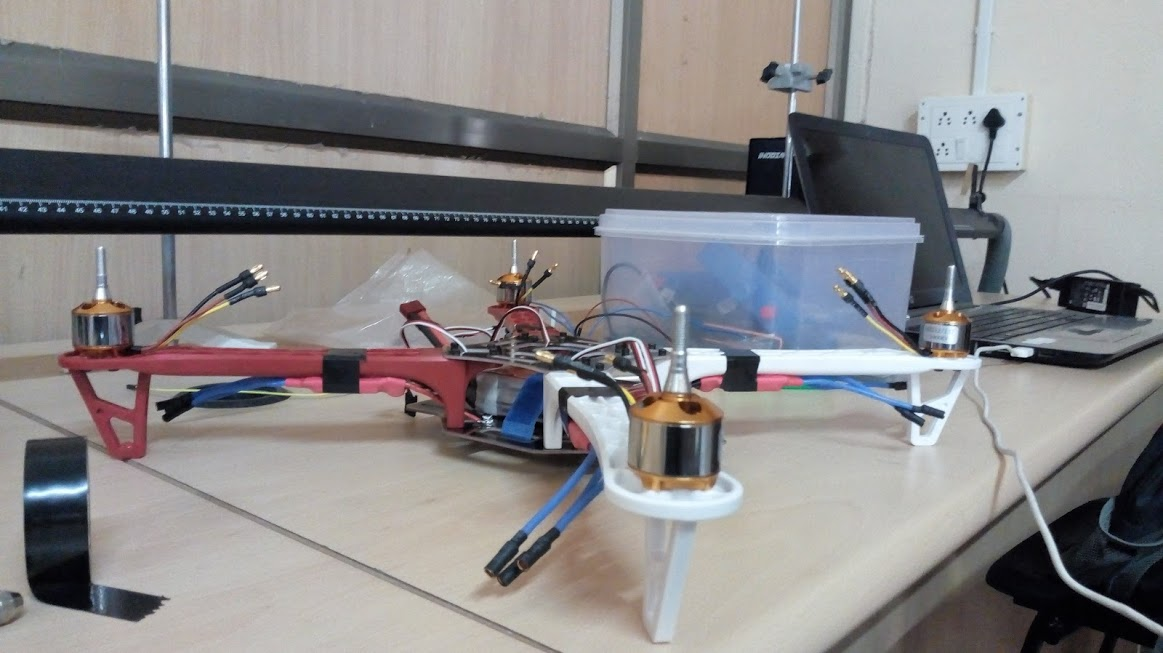
\includegraphics[width=0.5\textwidth]{motor_install}
\caption{Motors installed on to drone}
\end{figure}

\subsection{Adding KK Board with proper configuration}
The first and foremost thing is when you are working with flight controller you need to remove all the propellers for safety. DO NOT install the propellers when any setting is done at flight controller for the first time. Once fix the propellers after all motor checking never remove them to get a tight grip. \\
    The first thing to do is to set up the flight controller. Connect the battery to the base with the help of connector which we solder onto the base then flight controller will starts. Then we firstly check for sensors that all the sensors are working properly or not. For that go to Menu -> Sensor Test and check if all the values of Gyroscope and Accelerometer are working OK or not. We got the OK message across the board that means all the sensors are working properly. \\
    The next thing is accelerometer calibration it takes 5 seconds to calibrate and shows OK message with X and Y values. We do it because most of ESCs need to know the minimum and maximum PWM(Pulse Width Modulation is radio receiver protocol used to transfer data from Rx to Flight Controller) values that the flight controller will send. Then we went for mode setting and just verify that Link and Roll Pitch are YES. Now we are going to go over miscellaneous setting and make sure that Height Dampening set to zero. This feature tries to maintain altitude when the aircraft is pitching forward by regulating throttle. Experienced pilots do this automatically so that’s why it more suits for beginners than it is for advanced pilots. Then just one below that we changed the Alarm 1/10 Volts, for 3S batteries which we have 10.5V is OK (3.5V/cell) so the value will be 105. \\
    Now next we went for Load Motor Layout and choose the quadcopter-x mode which is very fine then after confirm it shows the rotation of each motor either it is CW or ACW. So we set the motors and connects ESC accordingly. To confirm you just go to Show Motor Layout and it will display the current configuration of motors.\\
	After motor installation and checking their rotation we need to fix the vibration which is generated by motors. Due to the small size of nut bolts, we can’t put the shock/vibration absorber in between the motor and the frame. So the other way to reduce motor vibration is to equalize the weight of the motor on every side. For that firstly we install the Vibration app which monitors the degree of vibration onto the frame by putting smartphone onto the frame, then the next problem is how to start the motor to do so we connect ESC of one motor into flight controller and power up the ESC by connecting battery. After taking raw measurements for motor vibration we cut the small piece of tape and paste it on the motor. Then we check the vibration. Due to cello tape, the weight of the motor is increased and it will definitely have an effect on the vibration, either it will increase or decrease so by trial and error method we find a suitable place on the motor whereby pasting tape vibration is reduced.

\begin{figure}[h]
\center
\begin{subfigure}[hb]{0.3\textwidth}
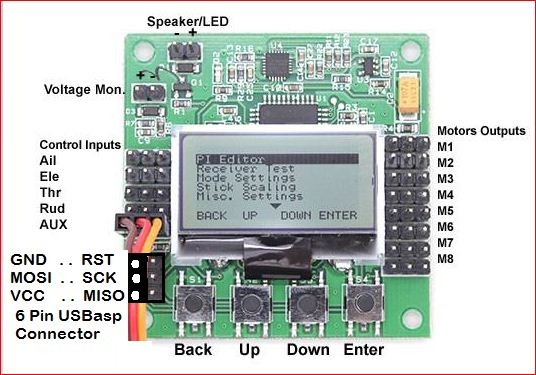
\includegraphics[width=\textwidth]{kk_flight}
\caption{KK flight controller}
\end{subfigure}
\begin{subfigure}[hb]{0.3\textwidth}
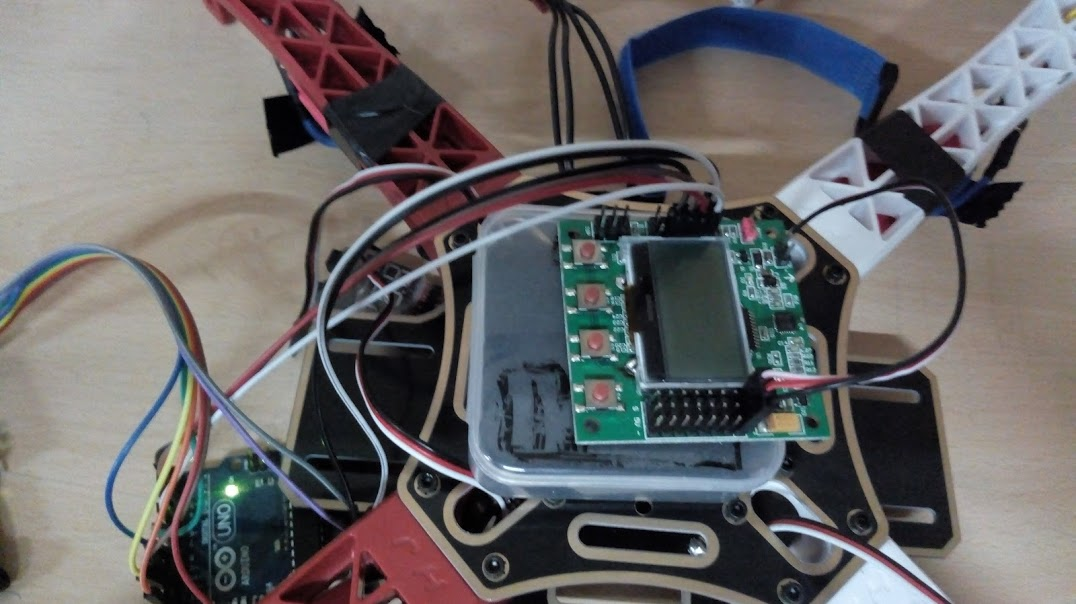
\includegraphics[width=\textwidth]{flight_controller}
\caption{Mounted flight controller on to the board}
\end{subfigure}
\end{figure}

%\begin{figure}
%\center
%\begin{subfigure}
%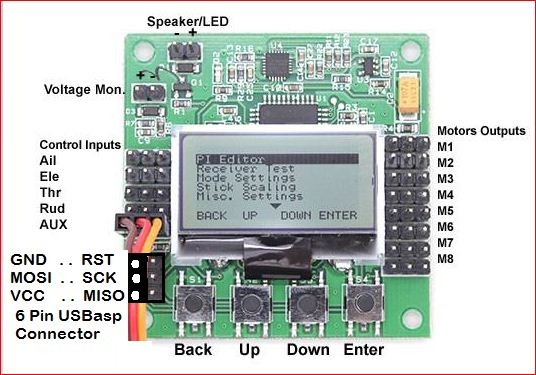
\includegraphics[width=0.35\textwidth]{kk_flight}
%\end{subfigure}
%\begin{subfigure}
%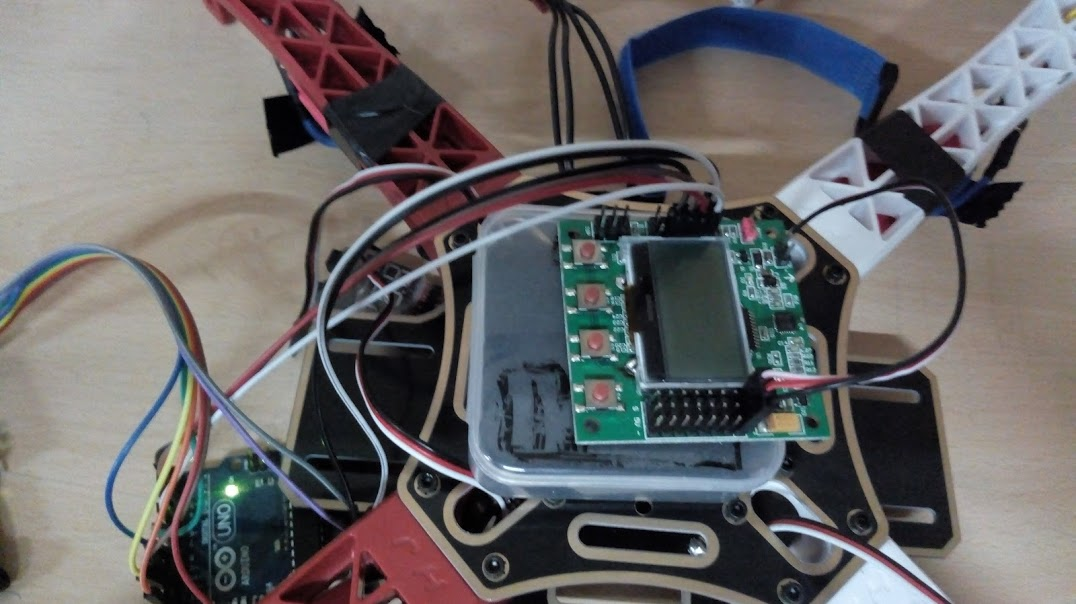
\includegraphics[width=0.45\textwidth]{flight_controller}
%\end{subfigure}
%\end{figure}

\subsection{Self-made Remote}
The next task is to create our own remote for that we have NRF modules and Joystick modules. We ordered NRF modules as transceivers i.e. the module is work as transmitter and receiver too. We write Arduino code for transmitter and receiver and using 2 Arduinos dumps the code into it. So our receiver contains Arduino and NRF module and transmitter contains Joysticks and Arduino. For the transmitter, there are 4 main values of joysticks named Throttle, Yaw, Pitch, and Roll. Throttle controls vertical up and down motion of the drone. Positive throttle will make the drone fly higher and negative throttle will make the drone fly lower. Yaw is the left and right rotation of the drone. Positive yaw will make the drone turn to the right and negative yaw will make the drone turn to the left. Pitch is the forward and backward tilt of the drone. The positive pitch will make the drone tilt and move forward and negative pitch will make the drone tilt and move backward. Roll is the side to side tilt of the drone. Positive roll will make the drone tilt to the right and negative roll will make the drone tilt to the left. We checked all the values in all cases i.e. maximum up maximum down and likewise and note down the values into the code to give a stable nature to the drone.The maximum values go to 255 and minimum goes to 0 and in the free position, it will be at 127. From the above analysis, we got to know that our modules are working properly and now we can bind transmitter and receiver. \\

\begin{figure}[h]
\center
\begin{subfigure}[hb]{0.2\textwidth}
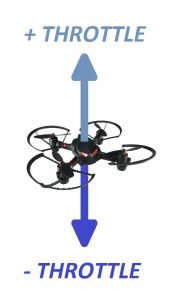
\includegraphics[width=\textwidth]{Throttle}
\caption{Throttle}
\end{subfigure}
\begin{subfigure}[hb]{0.2\textwidth}
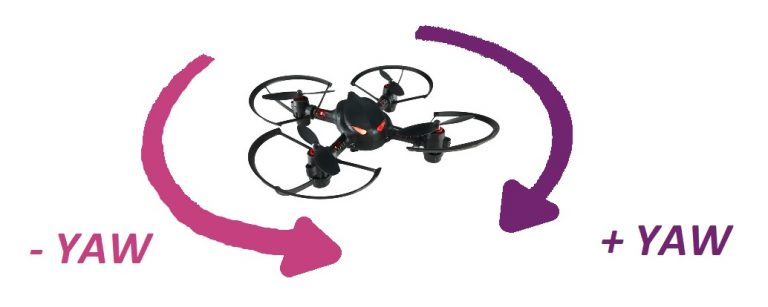
\includegraphics[width=\textwidth]{Yaw}
\caption{Yaw}
\end{subfigure}
\begin{subfigure}[hb]{0.2\textwidth}
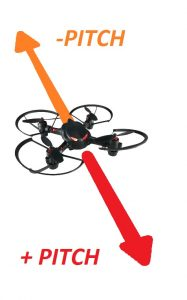
\includegraphics[width=\textwidth]{Pitch}
\caption{Pitch}
\end{subfigure}
\begin{subfigure}[hb]{0.2\textwidth}
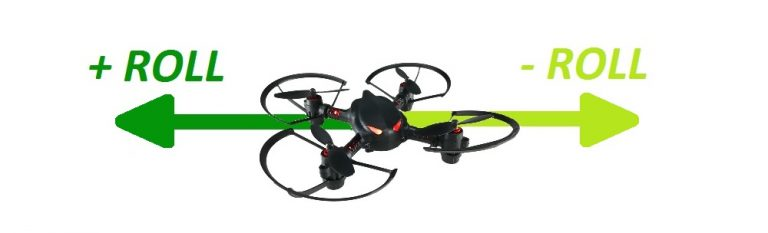
\includegraphics[width=\textwidth]{Roll}
\caption{Roll}
\end{subfigure}
\caption{Quadcopter axis of rotation}
\end{figure}
%
%\begin{figure}
%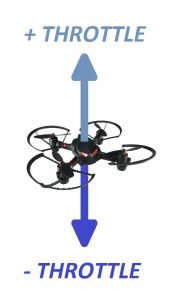
\includegraphics[width=0.20\textwidth]{Throttle}
%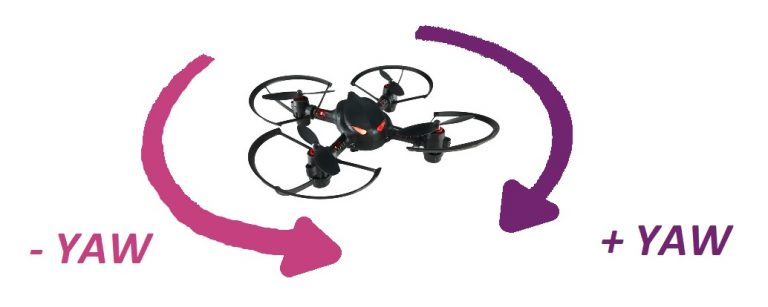
\includegraphics[width=0.35\textwidth]{Yaw}
%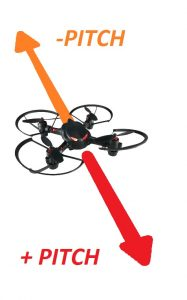
\includegraphics[width=0.20\textwidth]{Pitch}
%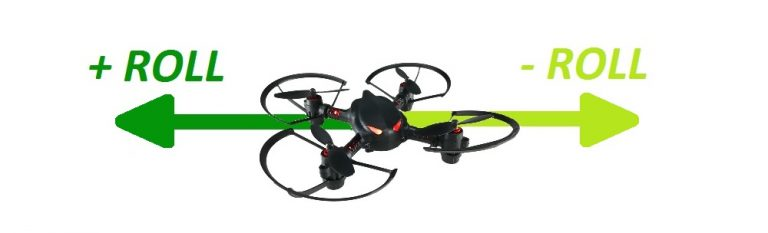
\includegraphics[width=0.35\textwidth]{Roll}
%\end{figure}
Here we only need to set the flight controller based on the receiver. First of all, we set all the four values i.e. Throttle, Yaw, Pitch, Roll to zero so that we get stable configuration while taking flight. Now for make your drone ready for flight you need to armed it then it will receive the signal and work accordingly but due to handmade remote we didn’t get how to armed it so for check of throttle value we just press the first and last button of flight controller and then give the power to drone the effect of it is the drone starts receiving the throttle value and we are able to check that signal is receiving correctly. Then the problem is we, not every time press the buttons while armed the drone so we need to operate it through remote so after a lot of searches we came across a solution and the solution is to arm your drone you need to pull throttle to left side downwards and to disarm it pull throttle to right side downward. After it we successfully able to change throttle value from remote itself.

\begin{figure}[h]
\center
\begin{subfigure}[hb]{0.3\textwidth}
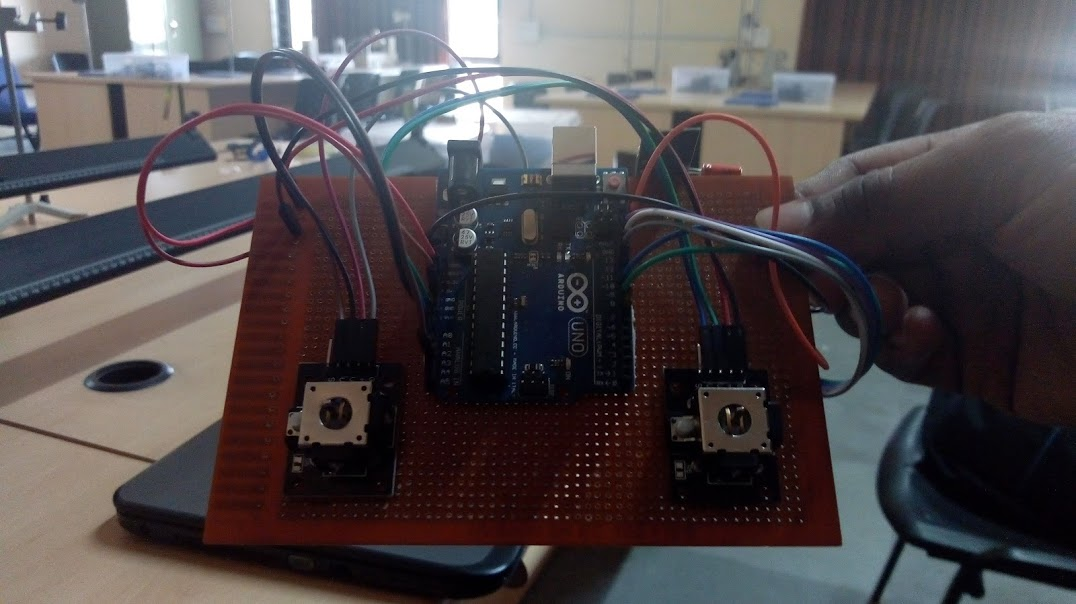
\includegraphics[width=\textwidth, height=8cm]{remote}
\caption{Self-made remote}
\end{subfigure}
\begin{subfigure}[hb]{0.3\textwidth}
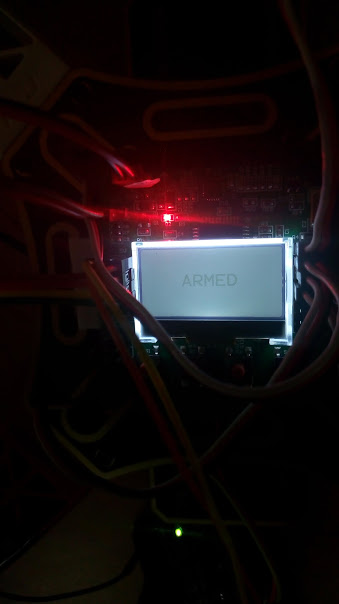
\includegraphics[width=\textwidth]{armed}
\caption{Armed position of the drone}
\end{subfigure}
\begin{subfigure}[hb]{0.3\textwidth}
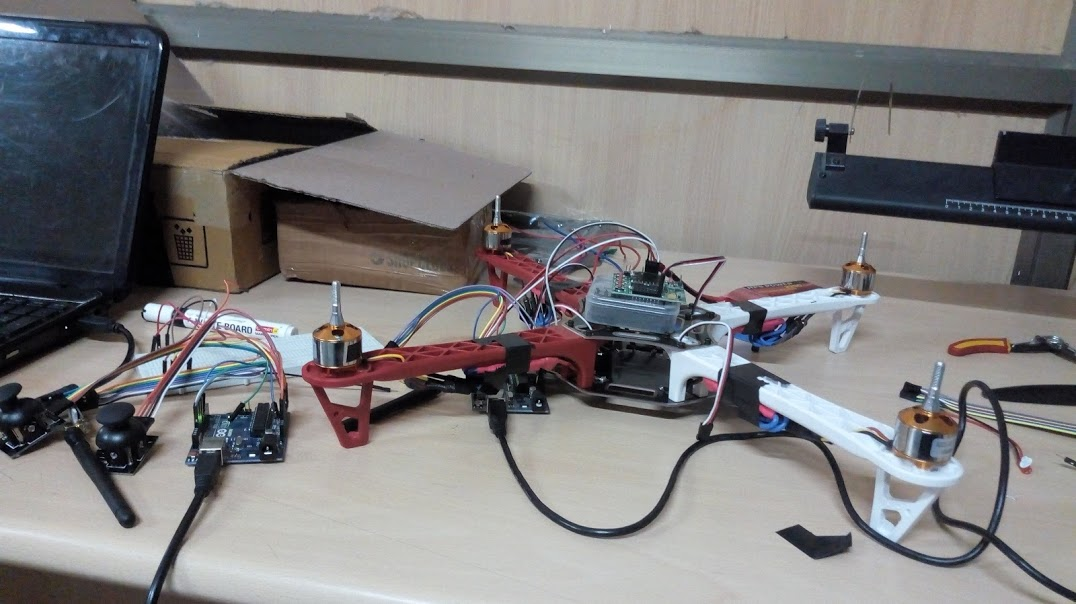
\includegraphics[width=\textwidth, height=8cm]{trans}
\caption{Complete view of transmitter and receiver}
\end{subfigure}
\end{figure}

%\begin{figure}
%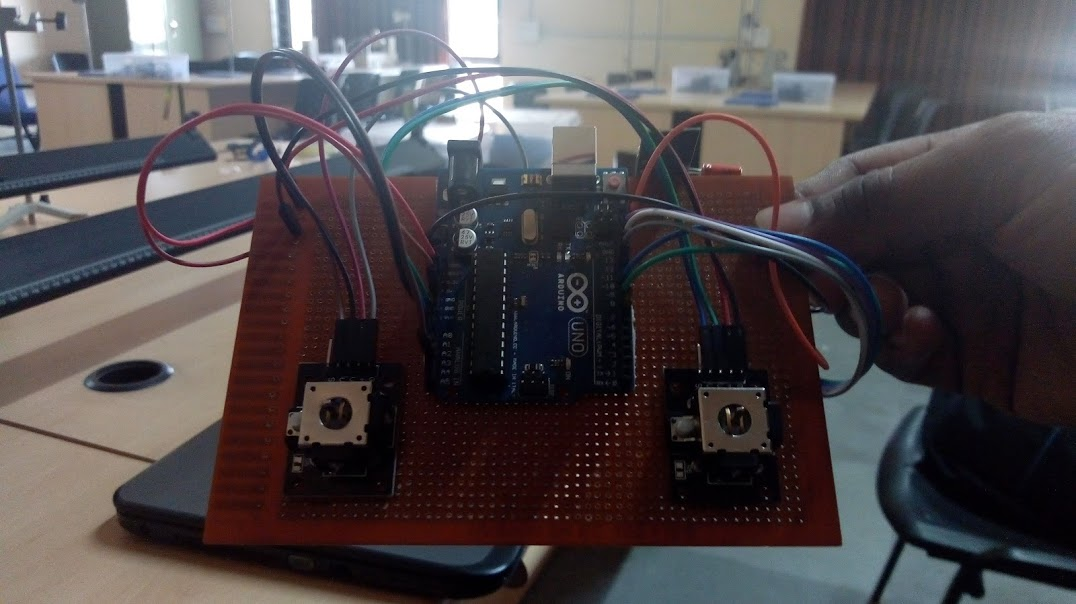
\includegraphics[width=0.38\textwidth]{remote}
%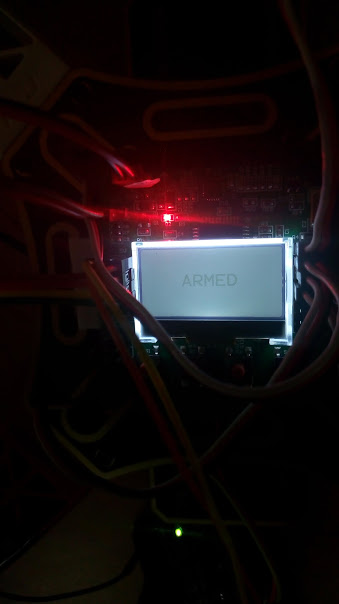
\includegraphics[width=0.25\textwidth]{armed}
%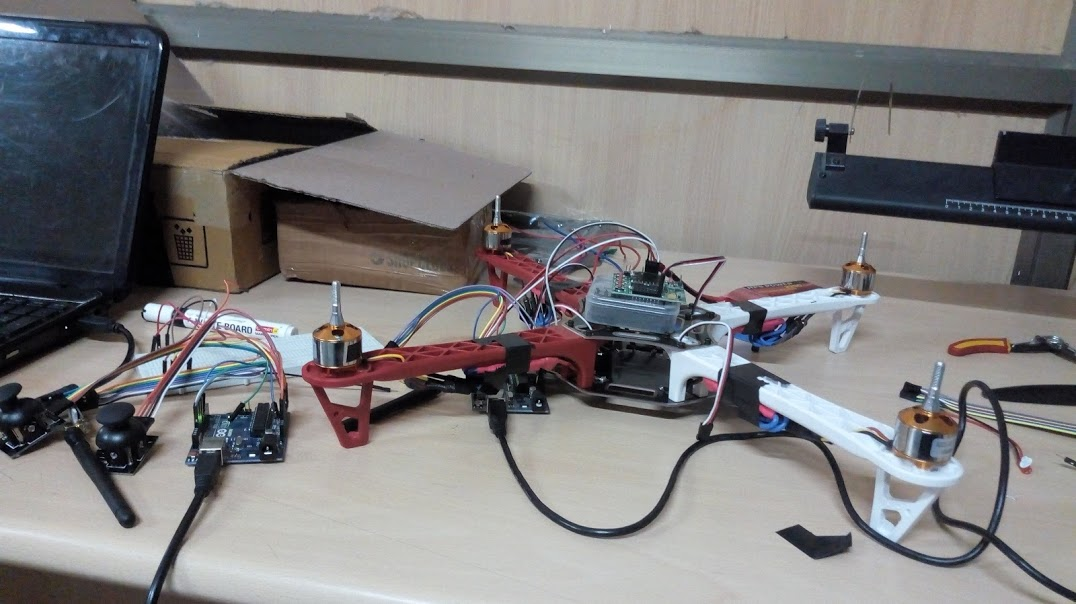
\includegraphics[width=0.35\textwidth]{trans}
%\end{figure}

\subsection{Adding Propellers}

First of all, we make sure that quadcopter switched off. For safety dis-arm it. After cross-check align it up (a threaded bolt with thick base). The long has to tight enough to make sure it will not loose and come out. Now when we open a pack of propellers there is a pack of spaces came with propellers. It is to fit the propeller with your motor. Try to choose the biggest which exactly fits into the motor. After inserting propellers tighten the cap. The main thing to notice is the direction of propellers must be same as motor configuration. To know which is clockwise and which is anti-clockwise the shape of prop gives the solution. 'L' shaped props are CW and vice-versa.\\
\begin{figure}[h]
\center
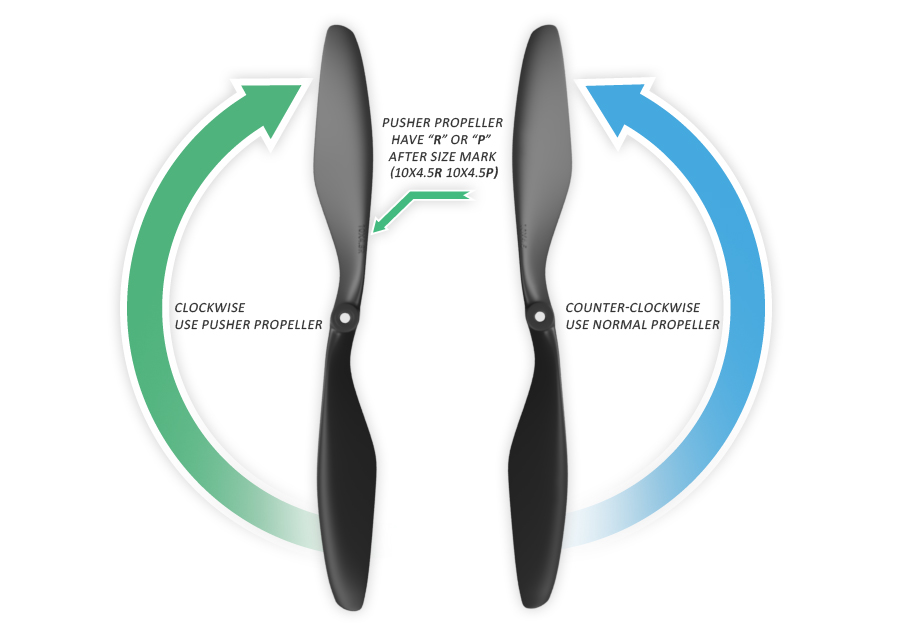
\includegraphics[width=0.5\textwidth]{props}
\caption{propeller's direction}
\end{figure}

%
%The reporting on the investigation shall be presented in one or more chapters
%with appropriate chapter titles.
%\begin{enumerate}
% \item 
%\item Due importance shall be given to experimental setups, procedures
%adopted, techniques developed, methodologies developed and adopted.
%\item While important derivations/formulae should normally be presented in
%the text of these chapters, extensive and long treatments, copious details
%and tedious information, detailed results in tabular and graphical forms
%may be presented in Appendices. Representative data in table and figures
%may, however, be included in appropriate chapters.
%\item Figures and tables should be presented immediately following their first
%mention in the text. Short tables and figures (say, less than half the
%writing area of the page) should be presented within the text, while large
%table and figures may be presented on separate pages.
%\item Equations should form separate lines with appropriate paragraph
%separation above and below the equation line, with equation numbers
%flushed to the right.
%
%\end{enumerate}

\section{Procedure for Home Automation}
Before starting the procedure lets take a look on block diagram:
\begin{figure}[h]
\center
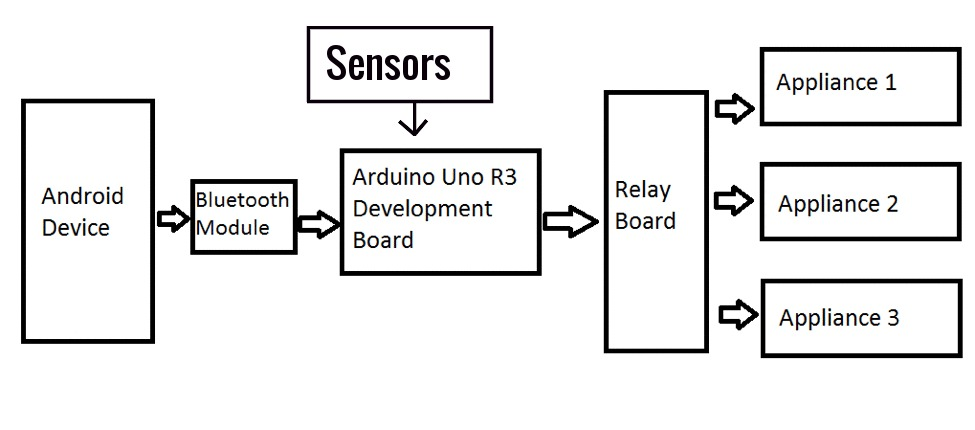
\includegraphics[width=0.8\textwidth]{block_diagram}
\caption{Block diagram for Home Automation}
\end{figure}

\subsection{Circuit Design}
The circuit design for home automation is very simple and its explained below:
\begin{itemize}
\item We have 4 appliances and those are connected to four electric switches in switch board.
\item Then take a 4-channel relay module and connect its pin to switches wire and another 4 pins are connected to Arduino port.
\item We are using two sensors namely Motion sensor and Temperature \& Humidity sensor.
\item These sensors are connected to Arduino with dedicated pins.
\item One Bluetooth module is connected for communication if required. 
\end{itemize}

\subsection{Working Process}
When the power is turned ON the connection LED on Bluetooth module starts blinking. Then we need to start the 'Bluetooth controller' app and get connected to the Bluetooth module. If the pairing is done then the LED becomes stable. Then in the app, we can control light, fan and other appliances.\\
But sometimes the pairing becomes time-consuming so here we fully-automate the appliances without any help of any smartphone. Basically, it works on sensors and based on the readings from sensors the relay work as a mediator and transfer the signals to the switchboard and appliances works accordingly.\\
\textbf{\textit{Caution:}} We should be very careful when using a relay with AC mains.

\end{chapter}

\begin{chapter}{Result}
\section{Quadcopter Result}
We successfully build a working drone which is able to monitor the surveillance of any area. The remote control made up of Arduino, joystick and NRF module is replaceable to any other well designed remote to a greater extent.\\
\begin{figure}[h]
\center
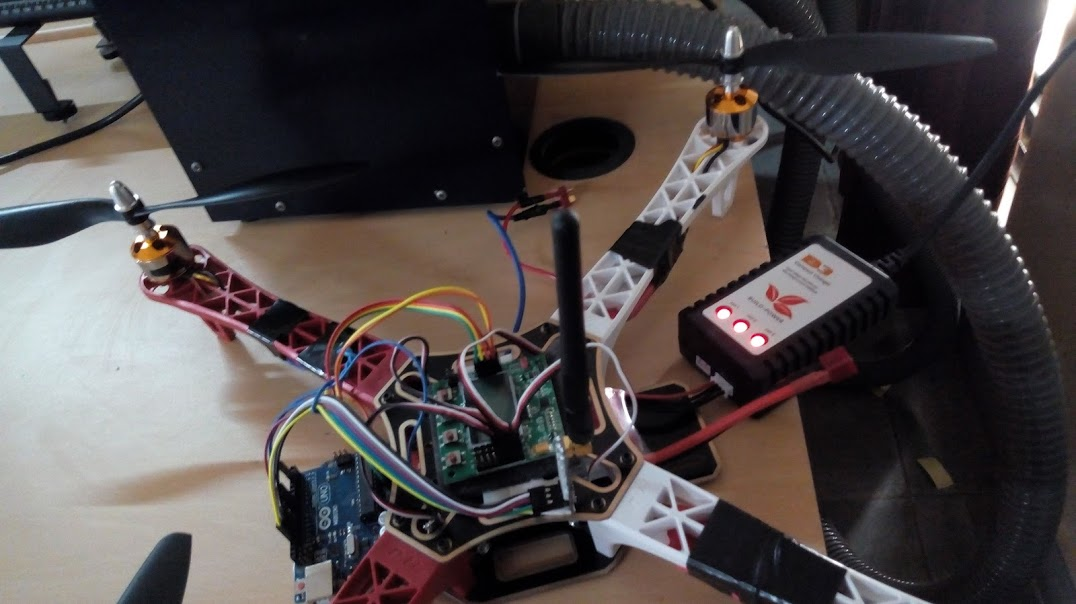
\includegraphics[width=0.45\textwidth]{final_drone}
\caption{Final drone as a product}
\end{figure}


%This shall form the penultimate chapter of the project report and shall include a
%thorough evaluation of the investigation carried out and bring out the
%contributions from the study. The discussion shall logically lead to inferences
%and conclusions as well as scope for possible further future work. 

%\begin{figure}
%
%\end{figure}

\section{Home Automation Result}
We are able to build an automated environment which can automatically switch ON the fans and light as the person enters the room and switch OFF as it exits the room. The camera mounted in the room is works as surveillance system which keep an eye on room 24x7.

\end{chapter}

\begin{chapter}{Conclusions}
\section{Qaudcopter-}

In this project, we mainly focus on new, cheap remote control which has all the functionalities same as commercial remote. Here are the differences between these remotes:\\

\begin{tabu} to \textwidth { | X[c] | X[c] | }
 \hline
 \textbf{Self-made Remote} & \textbf{Commertial Remote} \\
 \hline
 It costs around Rs.800 to Rs.900   & It costs around Rs.3300 to Rs.3500  \\
\hline
 It is easily portable & It is not easily portable.  \\
\hline
 It is small in size & It is comparitevly bigger than self-made remote.  \\
\hline
\end{tabu}


% This will be the final chapter of the project report. A brief report of the work
%carried out shall form the first part of the Chapter. Conclusions derived from the
%logical analysis presented in the Results and Discussions Chapter shall be
%presented and clearly enumerated, each point stated separately. Scope for future
%work should be stated lucidly in the last part of the chapter.

\section{Home Automation-}
We can successfully turn ON or OFF appliances remotely. This is just a basic idea of automation and can be upgraded further depending on its use.

\end{chapter}

\begin{chapter}{Future Scope}
 
\section{Quadcopter-}
\begin{itemize}
\item We are using a smartphone as camera onto drone but we can dedicate a camera and mount it onto the drone.
\item The range of NRF modules can be increase hence the altitude can go higher.
\item The model for face recognition used in our project has some limitations so by using better model efficiency can be increased.
\item The size of legs of the drone can be increased so that landing can be smooth and safe.
\end{itemize}

\section{Home Automation-}
\begin{itemize}
\item The home automation system can be expanded by including different sensors like light sensor, temperature sensor etc.
\item Additionally, we can also connect it to the Internet and control the home from any location via the Internet and monitor the safety.
\end{itemize}
  
\end{chapter}

\begin{thebibliography}{15}
\bibitem{book}
Building Your Own Drones: A Beginner's Guide to Drones, UAVs and ROVs
\\\textbf{\textit{John Baichtal}}
\\\textit{https://ptgmedia.pearsoncmg.com/images/9780789755988/samplepages/9780789755988.pdf}

\bibitem{docs}
Quadcopter Documentation
\\\textbf{\textit{Chris Laws}}
\\\textit{https://media.readthedocs.org/pdf/quadcopter/latest/quadcopter.pdf}

\bibitem{govt} 
Guidelines for obtaining Unique Identification Number (UIN) and Operation of Civil Unmanned Aircraft System (UAS)
\\\textit{http://www.dgca.nic.in}

\bibitem{wiki}
Wikipedia
\\\textit{http://www.wikipedia.com}



\end{thebibliography}

\end{document}
